% !TEX root = ../../../main.tex
% 来源：中学数学实验教材·第一册（代数）
% 章节：多项式的四则运算 / 一元多项式的除法
% 原始文件：4.tex，行 1698-1717
% 类型：tikz
% ---
    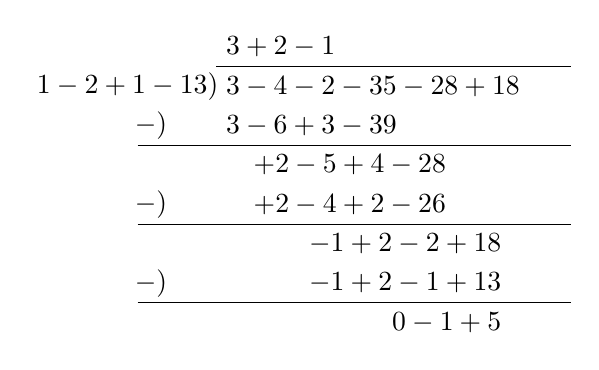
\begin{tikzpicture}
        \node at (0,0.5)[right]{$3+2-1$};
        \node at (0.15,0)[left]{$1-2+1-13)$};
        
        \node at (-.5,-0.5)[left]{$-)$};
        \node at (-.5,-1.5)[left]{$-)$};
        \node at (-.5,-2.5)[left]{$-)$};
        \draw (0,.25)--(4.5,.25);
    
        \node at (0,0)[right]{$3-4-2-35-28+18$};
    \node at (0,-.5)[right]{$3-6+3-39$};
    \draw (-1,-.75)--(4.5,-.75);
    \node at (0,-1)[right]{$\quad +2-5+4-28$};
    \node at (0,-1.5)[right]{$\quad +2-4+2-26$};
    \draw (-1,-1.75)--(4.5,-1.75);
    \node at (0,-2)[right]{$\qquad\quad -1+2-2+18$};
    \node at (0,-2.5)[right]{$\qquad\quad -1+2-1+13$};
    \draw (-1,-2.75)--(4.5,-2.75);
    \node at (0,-3)[right]{$\qquad\qquad\qquad 0-1+5$};
    \end{tikzpicture}  
